\documentclass[10pt,a4paper]{article}
\usepackage[utf8]{inputenc}
\usepackage[spanish]{babel}
\usepackage{amsmath}
\usepackage{amsfonts}
\usepackage{amssymb}
\usepackage{makeidx}
\usepackage{graphicx}
\usepackage{lmodern}
\usepackage{kpfonts}
\usepackage[left=2cm,right=2cm,top=2cm,bottom=2cm]{geometry}
\begin{document}
\begin{center}

\includegraphics[scale=0.2]{imagenes/upzmg.png} 
\end{center}
\large \huge Fabian canales ochoa, ING. Mecatroica 7-A \\ \\
\large \huge \textbf{Descripcion de la parametrizacion de rotaciones de acuerdo a los angulos de Euler.
} \\ \\
\Large  Puede demostrarse que cualquier rotación de un sólido puede expresarse como la composición de tres rotaciones elementales alrededor de ejes diferentes (no necesariamente ortogonales). A su vez, estas rotaciones pueden considerarse en torno a unos ejes fijos o en torno a unos ejes intrínsecos. Aquí consideraremos la segunda opción, es decir, especificaremos una composición de rotaciones que nos llevarán desde un sistema exterior considerado fijo (“sólido 1”) hasta un sistema ligado al sólido (“sólido 4”) mediante sólidos intermedios. Para ello: \\ \\
• primero efectuamos una rotación de un ángulo en torno a un eje del sólido 1 que nos lleva a un sólido intermedio “2”.\\
  •A continuación rotamos un ángulo  en torno a un eje del sólido 2, que nos lleva a un sólido intermedio “3”.\\
  •Por último, giramos un cierto ángulo  en torno a un eje del sólido 3, lo que nos lleva hasta el sólido móvil 4.
\Large Posición y matriz de rotación
Para obtener el resultado de la rotación, debemos ver qué posición ocupa en el sistema de referencia fijo un punto perteneciente al sólido. El vector de posición se escribirá con componentes diferentes en la base fija y en la base móvil, aunque el vector sea el mismo
donde, por ser un punto del sólido las componentes (X,Y,Z) son constantes. El problema se reduce entonces a relacionar los vectores de las bases. Para ello, componemos las tres rotaciones. en las siguientes iamgenes se ve las rotaciones graficamente (imagen 1.0 y 1.2)
\begin{center}
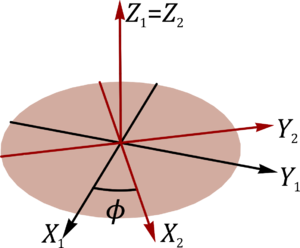
\includegraphics[scale=3.2]{imagenes/Angulos.png} imagen 1.0
\end{center}

\begin{center}
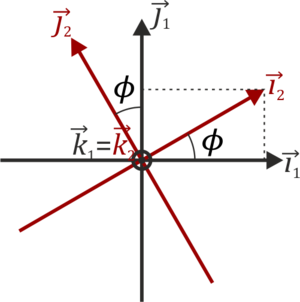
\includegraphics[scale=3.0]{imagenes/grafica.png} imagen 1.2
\end{center}
\Large Nutación
La segunda rotación consiste en el giro de un ángulo 0 alrededor del eje OX2 = OX3. A este eje, que no se ve modificado por la rotación, se lo denomina línea de nodos. Esta rotación nos lleva al sólido intermedio 3, cuya base se relaciona con la 2 por. Grafica mente se pueden visualizar en la imagen 2.0 y 2.1
\begin{center}
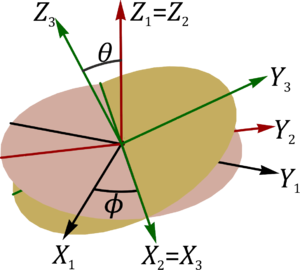
\includegraphics[scale=3.1]{imagenes/3D.png} imagen 2.0
\end{center}
\begin{center}
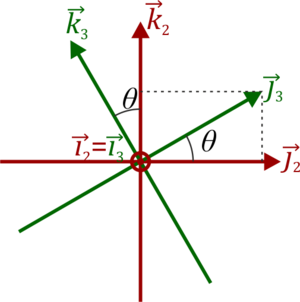
\includegraphics[scale=3.0]{imagenes/plano.png} imagen 2.1
\end{center}

\Large  Rotación propia
El tercer giro (rotación propia, rotación intrínseca o simplemente rotación en el contexto del movimiento terrestre) corresponde a un nuevo giro de un ángulo  alrededor del ángulo OZ3 = OZ4 (que no es el mismo, normalmente, que el OZ1 = OZ2). La relación entre las bases 3 y 4 es análoga a la que hay entre la 1 y la 2. Como se muestra en la imagen 3.0 y 3.1:
 \begin{center}
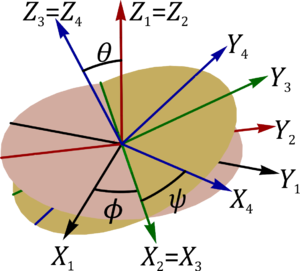
\includegraphics[scale=3.1]{imagenes/x.png} imagen 3.0
\end{center}
\begin{center}
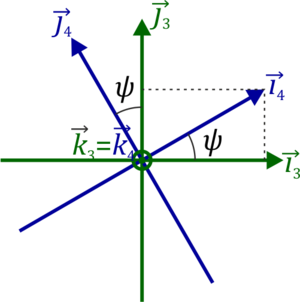
\includegraphics[scale=3.]{imagenes/j.png} imagen 3.1

\Large El origen de los nombres precesión, nutación y rotación procede del análisis del movimiento terrestre. La rotación es el movimiento alrededor del eje terrestre. La precesión es el lento movimiento de dicho eje, que provoca que la estrella situada en el polo norte celeste vaya cambiando en el tiempo. La nutación es el cambio en la inclinación del eje terrestre, que no siempre ha estado a 23°27' como actualmente.
\end{center}

\hspace{6cm}

\vspace{7cm}
{\Huge Referencias} \\
@article{del1993rotaciones,
  title={Rotaciones y espinores},
  author={Del Castillo, GF Torres},
  journal={Revista Mexicana de F{\'\i}sica},
  volume={40},
  number={1},
  pages={119--131},
  year={1993}
}
\end{document}